\chapter{UML diagramy a obrázky}
\section{Use cases}
\label{use_cases}

\begin{figure}[H]
\begin{center}
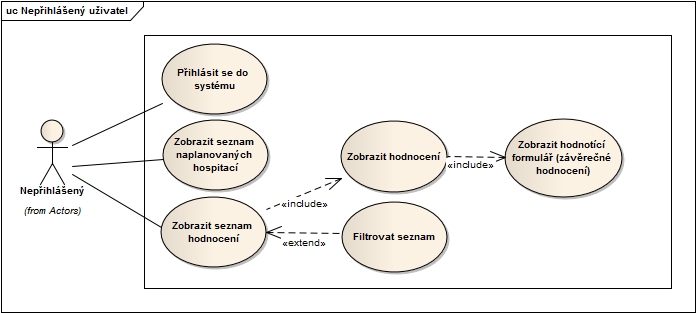
\includegraphics[width=12cm]{figures/actor_base}
\caption{Use case - nepřihlášený uživatel}
\label{fig:actor_base}
\end{center}
\end{figure}

\begin{figure}[H]
\begin{center}
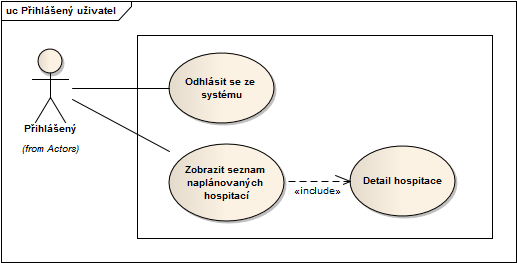
\includegraphics[width=12cm]{figures/actor_logged}
\caption{Use case - přihlášený uživatel}
\label{fig:actor_logged}
\end{center}
\end{figure}

\begin{figure}[H]
\begin{center}
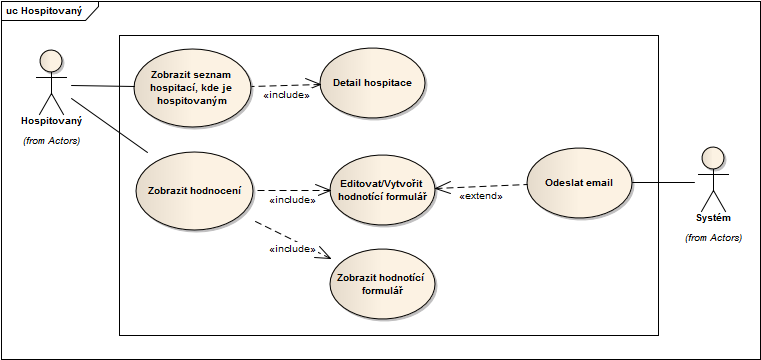
\includegraphics[width=12cm]{figures/actor_observed}
\caption{Use case - hospitovaný}
\label{fig:actor_observed}
\end{center}
\end{figure}

\begin{figure}[H]
\begin{center}
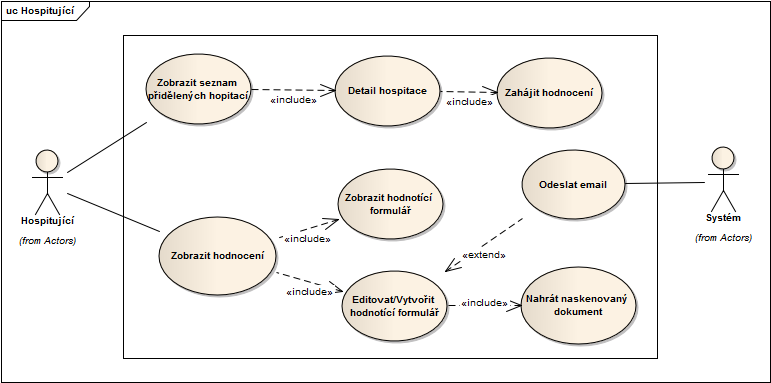
\includegraphics[width=12cm]{figures/actor_observer}
\caption{Use case - hospitující}
\label{fig:actor_observer}
\end{center}
\end{figure}

\begin{figure}[H]
\begin{center}
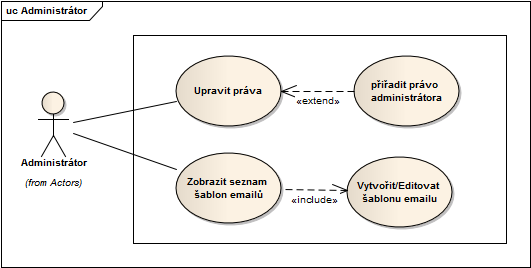
\includegraphics[width=12cm]{figures/actor_root}
\caption{Use case - administrátor}
\label{fig:actor_root}
\end{center}
\end{figure}

\begin{figure}[H]
\begin{center}
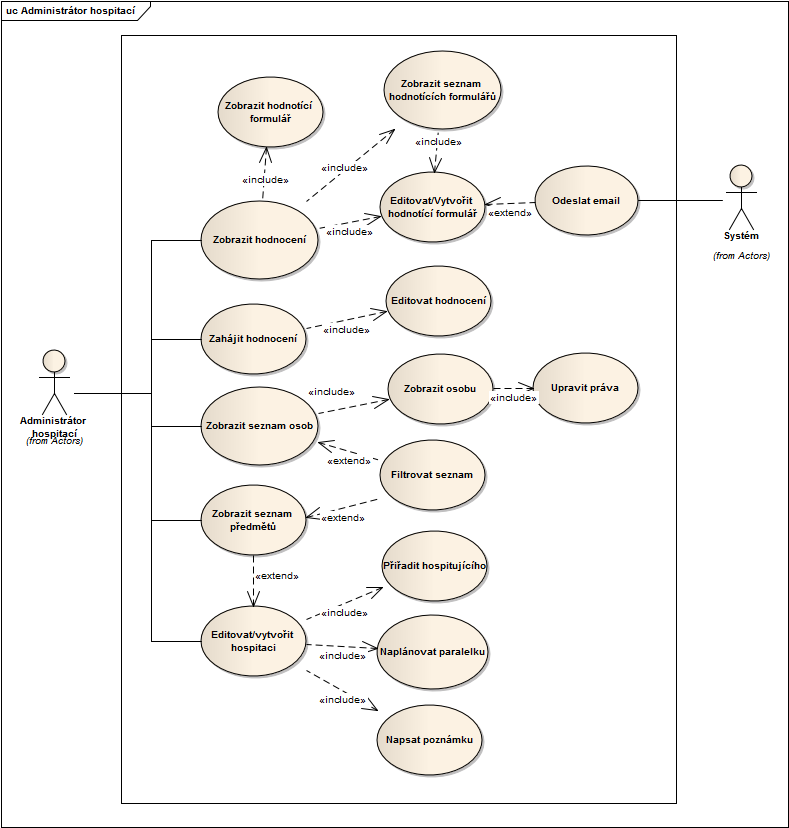
\includegraphics[width=14cm]{figures/actor_admin}
\caption{Use case - administrátor hospitací}
\label{fig:actor_admin}
\end{center}
\end{figure}


\chapter{Dynamické formuláře}
\label{sec:forms}
\begin{table}[h]
\begin{center}
\begin{tabular}{|l|c|l|}

\hline
\textbf{Typ} & \textbf{Návratová hodnota} & \textbf{Popis} \\ \hline
label &  & textový popisek \\\hline
integer & číslo & vstupní element pro čísla \\ \hline
text & text & formulář pro psaní textů \\\hline
text/file & text & formulář pro psaní textů s možností \\ & &  nahrání souboru s naskenovaným formulářem \\\hline
ranking\_table &  & tabulka pro hodnocení, může obsahovat několik \\ & & elementů typu \textit{ranking} \\\hline
column\_table & & tabulka do které se vkládají jiné elementy \\ & &  po sloupcích \\\hline
ranking & [A,B,C,D,E,F] & vstupní element pro zadávaní známkování  \\ & &   od A do F \\\hline
ranking\_scale & & tabulka s hodnotící stupnicí \\\hline
note & text & vstupní element pro napsání textové poznámky \\\hline

\end{tabular}
\caption{Seznam podporovaných typů elementů}
\label{tab:elements}
\end{center}
\end{table}

\begin{figure}[H]
\begin{center}
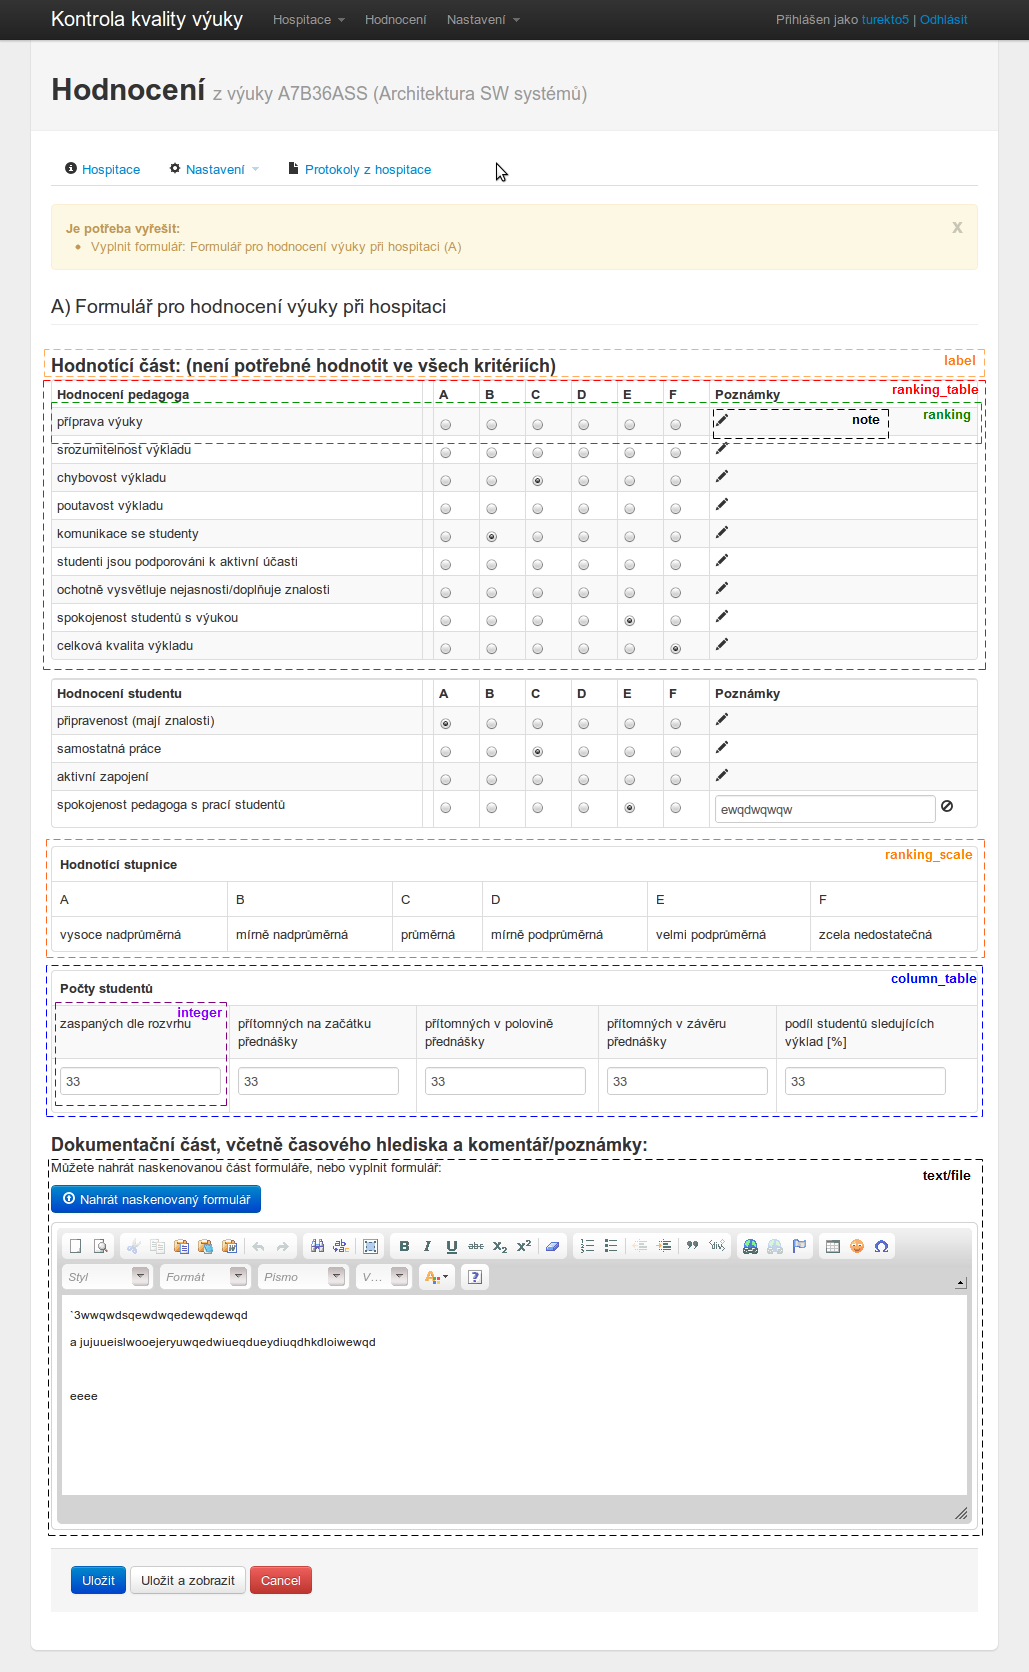
\includegraphics[width=14cm]{figures/form_A}
\caption{Hodnotící formulář A}
\label{fig:form_a}
\end{center}
\end{figure}

%*****************************************************************************
\chapter{Instalační a uživatelská příručka}
Instalační příručka je napsaná pro zprovoznění aplikace v prostředí development. Návod je určený pro operační systém Ubuntu 11.10. Pro zprovoznění aplikace je potřeba nainstalovat tyto programy:
\begin{itemize}
\item Ruby 1.9.3
\item RubyGems 1.8.13
\item Ruby on Rail 3.2.1
\item Databázový systém Mysql 5.5 nebo SQLite 3
\item Git
\end{itemize}

\section{Instalace}
Nejprve je potřeba nainstalovat platformu Ruby do systému. S ruby je potřeba nainstalovat i balík build-essential a git-core kvůli  knihovnám, které jsou potřeba pro zprovoznění aplikace. 

\begin{verbatim}
sudo apt-get install ruby1.9.3-full build-essential git-core
\end{verbatim}

Dále nainstalujte balíčkovací systém RubyGems a aktualizujte ho na poslední podporovanou verzi.
\begin{verbatim}
sudo apt-get install rubygems1.8
sudo gem update --system
\end{verbatim}

V poslední fázi je potřeba nainstalovat Ruby on Rails pomocí balíčkovacího programu rubygems.

\begin{verbatim}
sudo gem install rails
\end{verbatim}

Po nainstalovaní Ruby on Rails je potřeba doinstalovat všech závislostí aplikace. Nejprve je potřeba někam do systémů zkopírovat aplikaci např. do domovského adresáře. Ve všech dalších krocích se budeme pohybovat v adresáři aplikace. Druhý příkaz slouží k instalaci závislostí aplikace.

\begin{verbatim}
cd ~/Hospitace
bundle install
\end{verbatim}  

\section{Konfigurace a příprava aplikace}
Před spuštěním aplikace je důležité nastavit přístupové údaje k databázi. Nastavení databáze se nachází v souboru config/database.yml, který se nalézá v aplikaci. Pro zavedení databáze pak stačí jen spustit příkazy:

\begin{verbatim}
rake db:create
rake db:migrate
\end{verbatim}  

Máme vytvořenu databázi, ale je ji potřeba naplnit daty z KOSapi. Pro tento účel slouží příkaz:

\begin{verbatim}
rake import
\end{verbatim}

\section{Spuštění aplikace}
Pro spuštění aplikace použijte webový server Webrick, který je součástí Ruby on Rails. Po spuštění bude aplikace běžet na portu 3000.
Příkaz pro spuštění:
 
\begin{verbatim}
rails server
\end{verbatim}

%*****************************************************************************
\chapter{Obsah přiloženého CD}
\begin{figure}[h]
	\dirtree{%
		.1 /.
		.2 readme.txt\DTcomment{stručný popis obsahu CD}.
		.2 src/\DTcomment{zdrojové kódy aplikace}.
		.2 prototyp/\DTcomment{prototyp aplikace}.
		.3 src/\DTcomment{zdrojové kódy prototypu}.
		.3 BP.pdf\DTcomment{text prototypu ve formátu PDF}.
		.2 thesis/\DTcomment{zdrojová forma práce ve formátu
\LaTeX{}}.
 		.3 figures/\DTcomment{obrázky pro text práce}.
		.2 text/\DTcomment{zdrojová forma práce ve formátu}.
		.3 thesis.pdf\DTcomment{text práce ve formátu PDF}.
	}
	\caption{Obsah CD}
\label{tree:obsah_cd}
\end{figure}
%$ tree . >tree.txt
